\documentclass[tikz,border=3pt]{standalone}
\usepackage[utf8]{inputenc}
\usepackage[T1]{fontenc}
\usepackage{lmodern}
\renewcommand{\familydefault}{\sfdefault}
\usepackage{sansmath}\sansmath
\usepackage{chemfig}
\usepackage{pgfplots}\pgfplotsset{compat=1.18,/pgf/number format/use comma,/pgf/number format/1000 sep={.}}
\usetikzlibrary{arrows.meta,calc,positioning,decorations.pathmorphing,patterns}
% paleta del sitio
\definecolor{nar}{HTML}{E8680C}\definecolor{narc}{HTML}{FFB35C}\definecolor{hielo}{HTML}{FFF3E8}
\definecolor{tinta}{HTML}{1D1D1F}\definecolor{gris}{HTML}{6E6E73}\definecolor{lila}{HTML}{7C5CF0}
\definecolor{azul}{HTML}{2F6FD6}\definecolor{menta}{HTML}{17A673}\definecolor{coral}{HTML}{E8342A}
\begin{document}
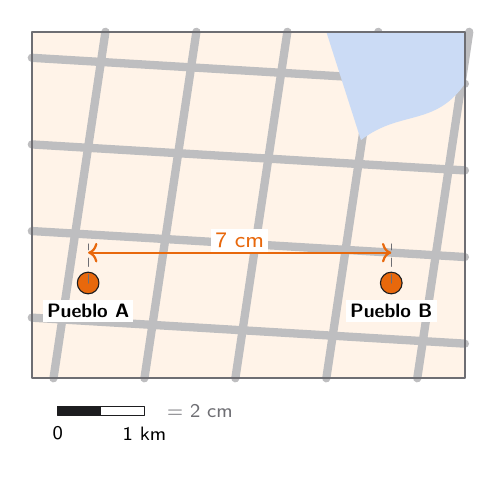
\begin{tikzpicture}[font=\small,x=0.55cm,y=0.55cm,line cap=round,line join=round,step={(1,1)}]
\fill[hielo] (0,0) rectangle (10,8);
\draw[gris!45,line width=3pt] (0.5,0)--(1.7,8);
\draw[gris!45,line width=3pt] (2.6,0)--(3.8,8);
\draw[gris!45,line width=3pt] (4.7,0)--(5.9,8);
\draw[gris!45,line width=3pt] (6.8,0)--(8.0,8);
\draw[gris!45,line width=3pt] (8.9,0)--(10.1,8);
\draw[gris!45,line width=3pt] (0,1.4)--(10,0.7999999999999999);
\draw[gris!45,line width=3pt] (0,3.4)--(10,2.8);
\draw[gris!45,line width=3pt] (0,5.4)--(10,4.800000000000001);
\draw[gris!45,line width=3pt] (0,7.4)--(10,6.800000000000001);
\fill[azul!25] (7.6,5.5) .. controls (8.5,6.2) and (9.3,5.8) .. (10,6.8)--(10,8)--(6.8,8)--cycle;
\draw[gris,thick] (0,0) rectangle (10,8);
\filldraw[fill=nar,draw=tinta] (1.3,2.2) circle (0.25); \node[font=\scriptsize\bfseries,fill=white,inner sep=1.5pt] at (1.3,1.55) {Pueblo A};
\filldraw[fill=nar,draw=tinta] (8.3,2.2) circle (0.25); \node[font=\scriptsize\bfseries,fill=white,inner sep=1.5pt] at (8.3,1.55) {Pueblo B};
\draw[gris,dashed] (1.3,2.2)--(1.3,3.1) (8.3,2.2)--(8.3,3.1); \draw[<->,nar,thick] (1.3,2.9)--(8.3,2.9) node[midway,above,fill=white,inner sep=1.5pt,font=\footnotesize] {7 cm};
\fill[white] (0.3,-1.6) rectangle (5.2,-0.3);
\fill[tinta] (0.6,-0.85) rectangle (1.6,-0.65); \draw[tinta] (0.6,-0.85) rectangle (2.6,-0.65);
\node[below,font=\scriptsize] at (0.6,-0.9) {0}; \node[below,font=\scriptsize] at (2.6,-0.9) {1 km};
\node[right,font=\scriptsize,text=gris] at (2.9,-0.75) {= 2 cm};
\end{tikzpicture}
\end{document}
